\chapter{Background and Literature Review}\label{chap:litreview}
\sloppy

This chapter summarizes the minimum background needed to motivate \textbf{ChromaGuide}: (i) what drives CRISPR-Cas9 on-target efficacy, (ii) how existing predictors model it, and (iii) the key gaps (context and calibrated uncertainty) addressed in this proposal.

\section{CRISPR-Cas9 on-target efficacy: essential biology}

\begin{figure}[htbp]
\centering
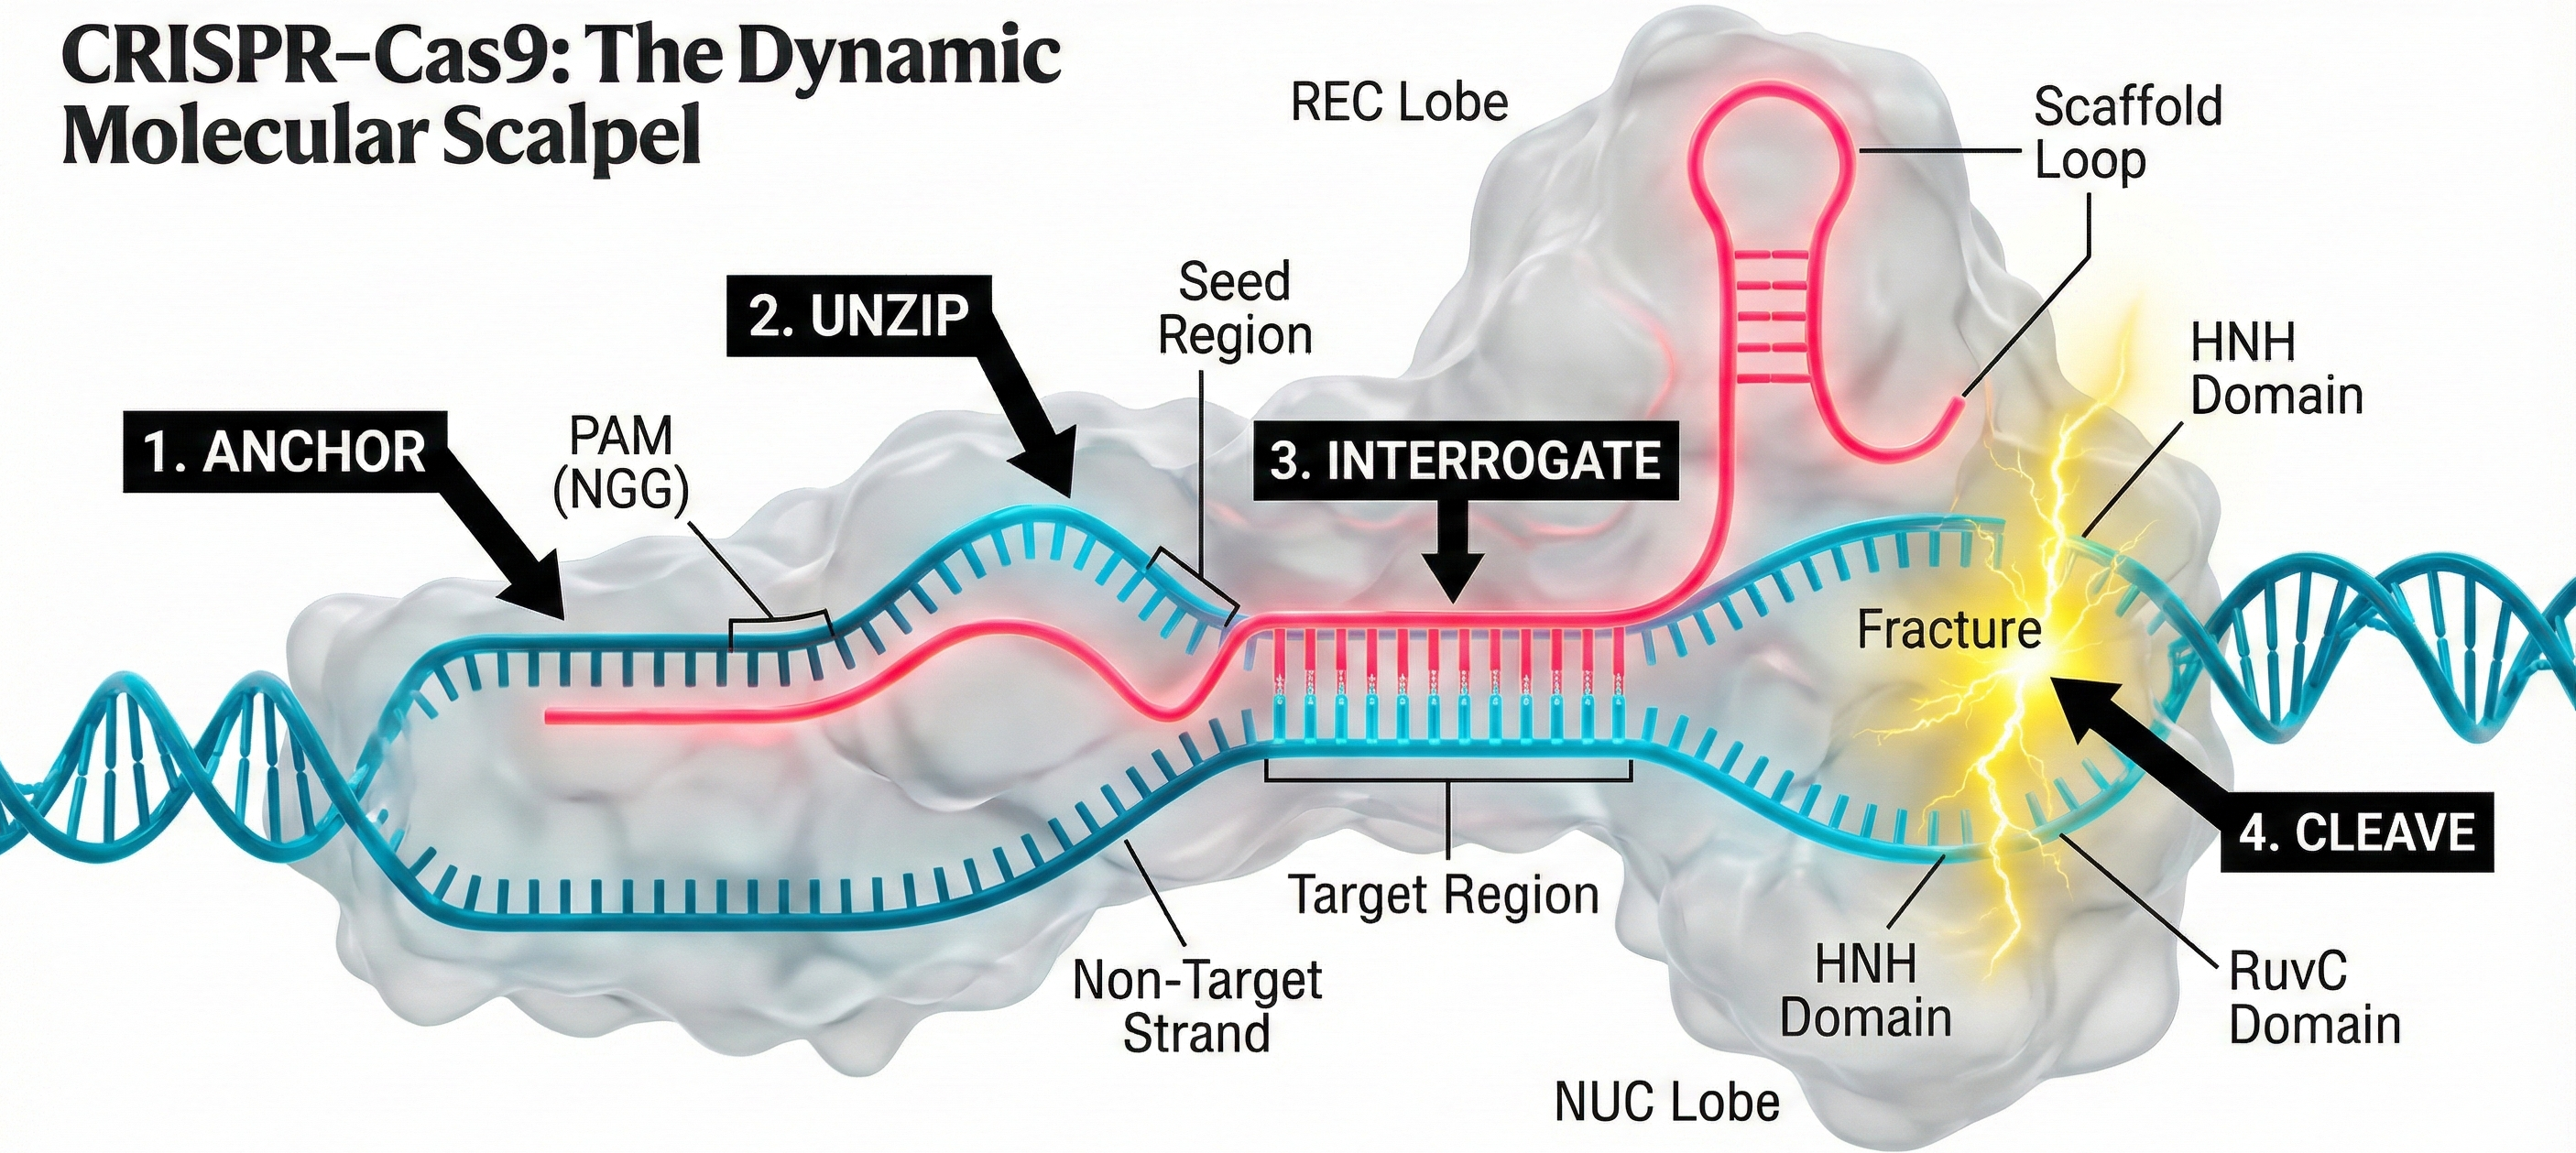
\includegraphics[width=0.9\textwidth]{Figs/CRISPR-Cas9.png}
\caption{CRISPR-Cas9 mechanism showing the four-step process: (A) PAM recognition and anchoring, (B) DNA unwinding, (C) seed region interrogation, and (D) target cleavage.}
\label{fig:crispr-mechanism}
\end{figure}

SpCas9 editing requires a \(\sim 20\)-nt protospacer and a nearby \PAM{} (typically NGG), followed by \CasNine\ binding and cleavage~\citep{jinek2012,hsu2014}. Observed efficacy varies with:
\begin{itemize}
\item \textbf{Sequence effects} (motifs/composition such as GC content).
\item \textbf{\gRNA\ structure/thermodynamics} that can influence guide availability.
\item \textbf{Chromatin accessibility/state} that modulates Cas9 access (e.g., nucleosome occupancy and accessibility)~\citep{horlbeck2016,isaac2016}.
\end{itemize}

\section{On-target predictors: what is typically modeled}

Most on-target predictors map a sequence representation (one-hot, engineered features, or pretrained embeddings) through a learned backbone (CNN/RNN/attention) to output an efficacy score. Representative baselines include DeepHF~\citep{wang2019}, DeepSpCas9~\citep{kim2019deepspcas9}, and ChromeCRISPR~\citep{daneshpajouh2025chromecrispr}. Context-aware models incorporate chromatin accessibility or related epigenomic signals when available, such as CRISPRon~\citep{xiang2021}.

\paragraph{Very recent (2025) on-target models (verified for this thesis scope).}
To keep this proposal concise while reflecting the latest literature, we highlight five 2025 models that motivate the ChromaGuide design space:
\begin{itemize}
\item \textbf{CRISPR\_\allowbreak HNN} (Li et al., 2025): a hybrid MSC +\allowbreak multi-head self-attention (MHSA) +\allowbreak BiGRU model for on-target activity prediction~\citep{li2025crisprhnn}.
\item \textbf{PLM-CRISPR} (Hou et al., 2025): cross-variant prediction that represents Cas9 variants using ESM2 protein language model embeddings~\citep{hou2025plmcrispr}.
\item \textbf{CRISPR-FMC} (Li et al., 2025): a dual-branch architecture for on-target prediction that fuses one-hot sequence features with pretrained RNA embeddings via cross-branch interactions~\citep{li2025crisprfmc}.
\item \textbf{Graph-CRISPR} (Jiang et al., 2025): a graph neural network model that integrates sequence and \sgRNA\ secondary structure features for on-target efficiency prediction~\citep{jiang2025graph-crispr}.
\item \textbf{ChromeCRISPR} (Daneshpajouh et al., 2025): a CNN+RNN (CNN--GRU) hybrid baseline for on-target prediction, emphasizing strong sequence modeling with lightweight auxiliary features (e.g., GC content)~\citep{daneshpajouh2025chromecrispr}.
\end{itemize}

\paragraph{Why protocol choice matters.}
Reported headline metrics remain sensitive to dataset choice and leakage/split design; realistic evaluation therefore requires gene-held-out and cross-domain (dataset/cell-line) stress tests.

% Table omitted for concision (models discussed in text).

\section{Off-target effects and prediction methods}

Off-target activity arises when a \gRNA\ partially matches additional genomic loci that are adjacent to a compatible \PAM{} and permissive to Cas9 binding and cleavage. Key determinants include (i) mismatch number and position (with the PAM-proximal ``seed'' typically less tolerant), (ii) mismatch type and local sequence context, (iii) DNA/RNA bulges, and (iv) chromatin accessibility and other epigenomic factors that can modulate cleavage probability at both intended and unintended loci.

\paragraph{Experimental profiling of off-targets.}
Genome-wide assays such as GUIDE-seq provide empirical off-target site lists and approximate relative activities, and are commonly used to benchmark computational predictors and guide model training/evaluation~\citep{tsai2015guideseq}.

\paragraph{Four families of computational methods.}
Off-target prediction methods can be grouped into:
\begin{enumerate}
\item \textbf{Alignment-based:} enumerate candidate off-target loci by genome-wide approximate matching under PAM and mismatch/bulge constraints (e.g., Cas-OFFinder)~\citep{bae2014casoffinder}.
\item \textbf{Formula-based:} compute mismatch-position-weighted scores (e.g., MIT score, CFD score) and aggregate them into guide-level specificity estimates (often used in pipelines such as CRISPOR)~\citep{doench2016,haeussler2016}.
\item \textbf{Energy-based:} approximate Cas9--\gRNA--DNA binding/cleavage energetics to score the likelihood of cleavage.
\item \textbf{Deep learning / foundation models:} learn site-level cleavage probabilities directly from \sgRNA\--target pairs, optionally integrating epigenomic context (e.g., DeepCRISPR, CCLMoff, DNABERT-Epi)~\citep{chuai2018,du2025cclmoff,kimata2025dnabertepi}.
\end{enumerate}

\paragraph{Recent SOTA: CCLMoff (Du et al., 2025).}
Du et al. introduced \textbf{CCLMoff}, a transformer-based off-target predictor that incorporates a pretrained RNA language model and reports AUROC $=0.996$ in a cross-dataset evaluation setting (train on CIRCLE-seq, test on GUIDE-seq), outperforming a range of prior deep learning baselines~\citep{du2025cclmoff}.

\paragraph{Epigenomics-aware foundation model: DNABERT-Epi (Kimata \& Satou, 2025).}
Kimata and Satou introduced \textbf{DNABERT-Epi}, which fine-tunes a DNABERT foundation model and integrates epigenetic features (H3K4me3, H3K27ac, and ATAC-seq). They benchmark against five baselines across seven off-target datasets and report competitive or superior performance, highlighting the value of combining sequence pretraining with local chromatin context for off-target risk prediction~\citep{kimata2025dnabertepi}.

\section{\sgRNA\ design principles and tools}

Practical \sgRNA\ design aims to select guides with high on-target activity while controlling off-target risk, under hard constraints such as PAM availability and experiment-specific requirements (e.g., U6 promoter compatibility). This is commonly operationalized as (i) generating candidate guides at a locus, (ii) predicting on-target efficacy, (iii) screening/penalizing off-targets, and (iv) selecting a final guide under an explicit efficiency--specificity trade-off.

\paragraph{Taxonomy of on-target predictors.}
On-target efficiency models can be grouped into:
\begin{itemize}
\item \textbf{Conventional ML:} feature-engineered models such as Azimuth/Rule Set 2~\citep{doench2016}.
\item \textbf{Deep learning / pretrained models:} sequence models that learn representations directly from data, sometimes augmented with thermodynamic/structural/epigenomic signals or pretrained embeddings (e.g., CRISPRon, DeepHF, DeepSpCas9, CRISPR\_HNN, CRISPR-FMC, Graph-CRISPR, PLM-CRISPR)~\citep{xiang2021,wang2019,kim2019deepspcas9,li2025crisprhnn,li2025crisprfmc,jiang2025graph-crispr,hou2025plmcrispr}.
\end{itemize}

\begin{sloppypar}
\paragraph{Anchor models and benchmarks.}
Classic deep learning baselines remain widely used: CRISPRon~\citep{xiang2021}, DeepHF~\citep{wang2019}, and DeepSpCas9~\citep{kim2019deepspcas9}. A benchmark and ensemble study by Chen and Wang (Bioinformatics 2022) compared 17 published scoring algorithms across 16 datasets totaling $>90{,}000$ gRNAs and identifies CRISPRon, DeepSpCas9, and DeepHF as top-performing individual predictors, with ensemble approaches (e.g., sgDesigner and TSAM) also ranking strongly~\citep{chen2022ensemble}.
\end{sloppypar}

\paragraph{Very recent 2025 trends.}
Recent SOTA work emphasizes (i) hybrid local+global architectures with dynamic feature weighting (CRISPR\_HNN)~\citep{li2025crisprhnn}, (ii) pretrained embeddings and cross-modal fusion (CRISPR-FMC; Graph-CRISPR)~\citep{li2025crisprfmc,jiang2025graph-crispr}, and (iii) cross-variant generalization by integrating Cas9 variant representations from protein language models (PLM-CRISPR)~\citep{hou2025plmcrispr}.

\paragraph{Design tools.}
End-to-end design tools implement candidate enumeration and integrate on-target and off-target scoring (e.g., CRISPOR, CHOPCHOP), often with practical filters and batch scoring capabilities~\citep{haeussler2016,labun2016chopchop}.
